\documentclass[a4paper,11pt]{article}

%
% Do not change
\textheight = 220mm
\textwidth  = 150mm
\topmargin  = 10mm
\oddsidemargin  = 5.0mm
\evensidemargin = 5.0mm
\unitlength = 1mm


\usepackage[T1]{fontenc} % Use latin1 font encoding

\usepackage[UKenglish]{babel} % If in Swedish

\usepackage{csquotes} % For blockquote
\usepackage{enumitem}

\usepackage[section]{placeins}
\usepackage{graphicx}
\graphicspath{{./figures/}}
\DeclareGraphicsExtensions{.pdf,.png}

\begin{document}

\let\rempage=\thepage
{
\renewcommand{\thepage}{\relax}
\begin{figure}
	
\includegraphics[width=0.18\textwidth]{mahlogo-name}
\end{figure}

\vspace*{-30mm}
\hfill\begin{minipage}[t]{10em}\large
Teknik och samh�lle\\
Datavetenskap
\end{minipage}

\vspace*{45mm}
\begin{center}
{\bf\large
Examensarbete 

\small
15 h�gskolepo�ng, grundniv�
}

\vspace*{25mm}
\LARGE

The differences in requirement elicitation between community- and firm-driven open source software projects on Github.

\vspace*{8mm}
\large

Examensarbetets titel p� svenska %TODO

\vspace*{12mm}
\Large
%
% Author names
Teddy Andersson\\
Filip Harald

\vspace*{30mm}
\large
% picture TODO?
\end{center}

\vfill
\hspace*{-10mm}%
\begin{minipage}[t]{20em}
%
% Fill in correct data for you
Examen:~kandidatexamen 180~hp
\\
Huvudomr�de:~datavetenskap
\\
Program:~systemutvecklare
\\
Datum f�r slutseminarium:~2016-xx-xx %TODO
\end{minipage}
\hfill
\begin{minipage}[t]{20em}
Handledare: Nancy Russo
\\
Assisterande handledare: Aleksander Fabijan
\\
Examinator: Mr. X
\end{minipage}

\newpage

\mbox{}

\newpage

\section*{Sammanfattning}

Text p� svenska\ldots

\newpage

\mbox{}

\newpage

\section*{Abstract}

Text in English\ldots

\newpage

\mbox{}

\newpage
\tableofcontents
\newpage
\ifodd\value{page}\else\mbox{}\newpage\fi
\setcounter{page}{1}
\renewcommand{\thepage}{\rempage}

\section{Introduction}
%Problem and challenges
Today there are several methods to choose from when you decide to develop or continue the integration of a software, and every method has it's own benefits and fits some projects better than others. During this process of deciding a method there are always a variety of factors that must be taken in consideration. One of these factors are elicitation of the development requirements, paragraphs that explains a functional or nonfunctional feature that the software must be able to handle, and this factor are effected of several challenges. First, software development is a knowledge-intensive activity with a large number of potentially confounding factors\cite{Curtis1986}, and this makes it difficult or impossible to discern the impact of commercial involvement. Second, to observe the impact of commercial involvement, it is important to compare the differences in contributions from developers, and to observe the work impact on projects over long period of time. Third, there is no easy way to learn companies, intentions motivating their involvement in the Open Source Software (OSS) community, and it is even more difficult to examine the effects of such involvement.

%Purpose
The challenges described above are key factors for this thesis purpose, to enlighten the decision of developing a software with a open source software (OSS) development method. By providing this information to governing bodies, regardless if there are a firm or a community backing the project, one important step in the development process could hopefully be made easier. This thesis will however not make a comparison between open source and proprietary software. Therefore this thesis will not either provide pros and cons of the transition from proprietary software to OSS. Bottom word the thesis will help governing bodies realize that OSS truly are commercial available.

%Contribution
As a result of this study we will have made the following three contributions. (a) As mentioned above our results can be used as support for a firm when deciding if they want to use OSS development. (b) When studying the characteristics of two OSS-projects the results will of course contribute to the general knowledge about OSS development. (c) The scripts we will develop and use to process the documented discussions(history) of the two projects.

%Approach
This thesis presents a comparative case study of differences in requirement elicitation between firm-driven and community-driven OSS projects on Github: Atom and Neovim. We address key questions about their differences towards each other overall and within the area of requirement elicitation, based on data gathered from Github. Based on the work of \cite{Mockus2002a} and \cite{Noll} we framed a number of hypotheses that we conjectured would be true generally of both development and requirement elicitation within the area of OSS-development.

\subsection{Background}

\begin{displayquote}
	A great babbling bazaar of differing agendas and approaches out of which a coherent and stable system could seemingly emerge only by a succession of miracles.
\end{displayquote}

%introduce the reader to the section
	%Introduce the reader to System Development
In the evolution of software development different types of methods have been used to manage initiation, planning, execution, monitoring and closeout of a software project. The project methods whom where first to adopt these phases are known as traditional development methods. The traditional development methods approach identifies a sequence of steps to be completed, where the work of a new step don't begin until the previous step is completed. However these project method was not optimal for software development, where the need of continuos integration is important.\cite{Jansson2015} Therefor on February 11?13\footnote{TODO}, 2001, at The Lodge at Snowbird ski resort in the Wasatch mountains of Utah, 17 people met to talk, ski, relax and try to find common ground. What emerged under this meeting was the Agile Software Development Alliance. From this alliance the Agile methods evolved based on a manifesto where the effort was to overcome perceived and actual weakness in conventional software engineering. This alliance wrote down the famous Agile Manifesto and their reason was simply to undercover better ways of developing software by doing it and helping others do it\cite{Fowler2001}. In contrast to the traditional methods the agile methods are based on incremental method managing the design and build activities of engineering\cite{Jansson2015} . Apart from the traditional and agile methods the open source software (OSS) development method started to received  a lot of attention in the late 90's. OSS development is the process by which open-source, or similar software whose source code is publicly available, is developed. These are software products available with its source code under a open-source license to study, change and improve its design. For this reason the OSS was in the late 90's characterized as a fundamental new way to develop software and was seen as a challenge to the commercial software business that did dominate the vast majority of the software market\cite{Mockus2002a}. But time have proven that OSS are a development method that can be applied on commercial software and maintain quality.  Examples of some popular open-source software products are Mozilla Firefox, Google Chromium, Android, LibreOffice and the Apache OpenOffice Suite. Open-source software development has been a large part of the creation of the World Wide Web as we know it, with Tim Berners-Lee contributing his HTML code development as the original platform upon which the internet is now built. \cite{http://www.wired.co.uk/article/tim-berners-lee}

	%TODO: More on the open source story

	%Introduce the reader to Community-driven projects and Requierment elicitaton
	
Regardless of the method a project choose to use in the develop a software system would most likeley need to handle requirements in one way or another. While traditional and agile requirements are elicitated from discussions with a client/customer OSS project handels the elicitation threw the users/developers that are involved in the OSS community. People in these communities cooperate via the Internet and never, or seldom, meet face to face. The number of developers can differ from a handful to thousands and are often geographically distributed. Developers voluntarily contributes to the software by implementing new features, fixing bugs and writing documentation \cite{Maccormack2006}. The key decisions in project driven OSS communities are taken by a central group of software developers (core developers). Beyond this central group, are the peripheral developers these are developers who intermittently submit code contributions (called patches). The core group reviews the patches before they are incorporated into the projects source code. \cite{Crowston2006}


%Introduce the reader to Firm-driven development
The Agile methods are popular to use in Software Companies for information systems development. Agile methods are claimed to encourage developers to be more flexible and efficient by means of arrangements in the development teams physical and social environment\cite{Jansson2015}. In recent years, however, we have seen a increased interest of using open source alongside with the Agile development\cite{Author2008,Jansson2015}. Big companies like Google have been striving towards a more open environment in both development projects but also in general work process\cite{How Google Works}\footnote{Fix a reference for the book, couldn't find a pdf version, but i have it in the bookshelf in the apartment //Teddy}. Alongside with an interest and momentum of OSS it is now also considered to be, in a commercial settings, a more viable approach\cite{Author2008}. From a commercial stand point OSS development also promises many advantages. Including reduced salary costs; reduced cycle time arising from' 'follow-the-sun'' software development; cross-site modularization of development work; access to a larger skilled developer pool; innovation and shared best practice; and closer proximity to customers\cite{Author2008}.\footnote{Include how open source with a firm in the background are structured}

\subsection{Related Work}
\label{related_work}
%Explain the context of the other two studies and their findings/limitations
In previous work within the area of OSS and requirement elicitation there are to highly relevant studies for this thesis. The first article\cite{Mockus2002a} presents two case studies of the development and maintance of major OSS projects: the Apache server and Mozilla. Where Audris Mokus, Roy T Fielding and James D Herbsleb adress key questions about the development process, and about the software that is the result of the processes. Based on results from a erlier study made on Apache, covered in the article A Case Study of Open Source software Development: the Apache server, they framed a number of hypotheses that they conjectured would be true generally of open source developments. The second case study in the article\cite{Mockus2002a} examined data from the Mozilla project based on the analyses and hypothesis that where framed from the Apache project.  Audris Mokus, Roy T Fielding and James D Herbsleb came to the conclusion that the essential differences in which elements of commercial and open source processes could be combined have to do with coordination, selection, and assignment of the work.\footnote{In need of further conclusion explanation?}
The second highly relevant article\cite{Noll} requirements elicitation in open source software development: a case study. John Noll and Wei-Ming Liu presents a case study of the OpenEMR, an open source project developing electronic medical record (EMR) software. Where the goal of the study was to understand how requirements are elicited, documented, agreed and validated in a small open source software project. The study did follow the approach of an earlier study of the Firefox web browser, a much wider project. The comparison between the both project showed that, smilar to Firefox, the majority of OpenEMR requirements are asserted by developers. Documentation was likewise informal, consisting mainly of archived discussions. Contributors to the OpenEMR project where end-user, in this case medical practitioners such as doctors  or clinic administrations, who use the product in their practices. The implication for software development in general is that developers can be a significant source of innovation.

%Communicate to the reader that what WE are doing has not been done just yet. 
The articles together summarize the differences between open-source projects in different aspects. Audris Mokus, Roy T Fielding and James D Herbsleb investigate two case studies from which they try to form theories on what it is that defines OSS-projects. They conclude the study by comparing their results with commercial, proprietary, projects\cite{Mockus2002a}. John Noll and Wei-Ming Liu on the other hand  investigate the differences in requirement elicitation between large and small OSS-projects\cite{Noll}. These project are the closest and most reliable sources we could find in the comparison with focus on the difference between requirement elicitation in firm driven OSS project and community driven OSS project.

%TODO: Shortly describe structure of report

\subsection{Research Question}
%Describe how this study will contribute to a solution or solve it completely
\begin{enumerate}[label=RQ\arabic*]
	\item \emph{What are the characteristics of community-driven OSS development?}
	\item \emph{What are the characteristics of firm-driven OSS development?}
	\item \emph{How can software companies benefit from engaging in corporate-driven OSS development?}\footnote{This question needs to be modified.}
\end{enumerate}
%-----------------------------------------------------------------------------------------------------------------------------------------------------------------------
\newpage
\section{Methodology}

%Descirbe what we want to research 
The purpose of this study is to compare the effects two different types of governing bodies, a firm or a non-profit community, have on OSS-projects. Given the nature of them both being OSS most of the information will publicly documented, including both code evolution and discussions between project participants. With these given conditions we've chosen to conduct a comparative case study on two OSS-projects, one of each type of governing bodies mentioned earlier.

% why not survey
With the given conditions mentioned in the previous paragraph one could argue that conducting a survey would be more suitable. However, such a survey would risk to miss out on detailed information that is unique for each project.

\subsection{Case Description}
This section describes the two projects that we have conducted our case studies on. The two projects we investigated, Atom and NeoVim,  are open-source texteditors, a program that are used for editing textfiles such as the source code of a software,  that are free too use and the source code from these projects are available too investigate on GitHub.

% In this section we will describe the two projects we intend to do our case studies on. First we describe Atom, then we describe NeoVim.
\subsubsection{Case 1: Atom}
%Explain Atom
Atom is a free and open-source text and source code editor for macOS, Linux and Microsoft Windows. The Atom project was initialised by Github on Github in August 14 2011 and have since then grown to be a very popular text editor for developers all around the world. The project have today a total of 349 contributors that have been made one or several contributions from the start of the project. Atom is licensed under the MIT license( A short and simple permissive license with conditions only requiring preservation of copyright and license notices. ). Github are still in control of the development process. Atom also have a huge amount extending packages developed by its own users under free software licenses and are community-built and maintained. Atom was released from beta, as version 1.0, on June 25, 2015. Its developers calls it "a hackable text editor for the 21st Century".\cite{atom_wp,atom_pp}


\subsubsection{Case 2: NeoVim}
\label{neo_vim}
%Explain Neovim
Neovim is a free and open-source text and source code editor for macOs, Linux and Microsoft Windows.  The Neovim project started in 2014 on Github, with some Vim community members offering early support of the high-level refactoring effort to provide better scripting, plugins, and integration with modern GUIs. Vim (Vi Improved) are a text editor who was first released in 1991 under a special license compatible with the GNU General Public License( a free, copyleft license for software and other kinds of works.) to be make creating and changing any kind of text very efficient. Neovim is therefor a refactor of Vim and strives to be a superset of Vim except for some intentionally-removed misfeatures. It is built for users who want the good parts of Vim, and more. The Neovim Project today have a total of 309 contributors that have been involved in writing code in one way or another. Neovim are driven by an independent community that are able to support the project through monthly subscriptions. Neovim had its first public released on 1 November 2015 \cite{neovim_wp,neovim_wiki}.

\subsubsection{Motivation for Selection of Cases}
\label{case_selection}
To ensure our results reflect only the requirement elicitation process of the projects we selected projects that are similar on other aspects. Especially on product type, project age and project size. both project develop a product that is classified as a text-editor. Atom has a more graphical user interface than Neovim, but they are still both used for the same purpose. The projects were created 5- (Atom) and 3- (Neovim) years ago. When comparing project size we used the data available on the main page for each project on Github\cite{atom_pp,neovim_pp} and also counted project LoC \footnote{Lines of Code, this is a common metric for determining how big a software is.} and amount of files. The data is presented in the table~\ref{tab:github_stats}.

TODO, should the numbers be rounded for easier comparison?
\begin{table}[h]
	\centering
	\begin{tabular}{ | l | c | c | c | c |}
		\hline
		\textbf{Data} 			& \textbf{Atom} 	& \textbf{Neovim}	& \textbf{Largest}	& \textbf{Difference}	\\\hline
		Contributors	 		& 349 		& 303 			& Atom			& 46				\\\hline
		Commits		 		& 31382 		& 7925 			& Atom			& 23457			\\\hline
		%Forks 				& 6218 		& 1586		 	&				& 4632			\\\hline
		%Stars 				& 35871	 	& 22114			&		 		& 13757			\\\hline
		%Watching			& 2021 		& 957			&		 		& 1064			\\\hline
		%Open Issues 			&1677 		& 599 			&				& 1078			\\\hline
		%Open Pull Requests 	& 105 		& 169 			&				& 64				\\\hline
		LoC 					& 57089		&  246741			& Neovim			& 189652			\\\hline
		Number of files 			& 388		& 579		 	& Neovim			& 191			\\
		\hline 
	\end{tabular}
	\caption{Project statistics found on Github as of March 2017\cite{atom_pp,neovim_pp}.}
	\label{tab:github_stats}
\end{table}

\FloatBarrier
We can identify three things\footnote{HELP! a better word than 'thing'} from the data: the projects are similar on the amount of contributors, Atom has a greater amount of commits and Neovim seems to be larger in terms of LoC and amount of files. Below we will address the two differences.

With Atom having more than 3 times as many commits as Neovim there is a significant difference. However the usage of how one would commit code could differ between the two projects. For example the amount of LoC committed could be approximately the same even if amount of commits differ.

The last, and perhaps most significant, is the difference in amount of LoC and files. As mentioned in section \ref{neo_vim} Neovim is a product that uses a lot of the functionality from Vim. The result of this is that Neovim has a lot of code which has been transferred from Vim. Vim has 328722 LoC and 230 files.

The two addressed differences were considered when constructing and conducting the case study. And even with these differences, Atom and Neovim are the most similar firm- and comunity-driven OSS projects of the ones investigated. Other candidates were, Google Chrome and Mozilla Firefox(difference in age and location of codebase) and Codelite instead of Neovim(Codelite was considerably smaller and older than Atom).

\subsection{Case Study}
%what is a case study?
In \cite{Oates2005} the author refers to a case study as being research strategy for which one tries to describe a case, or phenomenon, from within its natural context. Rather than just confirming a phenomenons existence, which could be done by for example conducting a survey, a case study aims to discover why it occurred. This is done, as a researcher, by aiming to give a detailed description of not just the phenomenon but also it's context. It is from the context the researcher can identify factors which might have caused the phenomenon to occur. The amount of factors varies from case to case and the probability of multiple causing factors should be taken into account.

%internet case studies
In \cite{Oates2005} the author says that case study can favourably be used when ''studying the 'life' on the Internet''. However the author mentions particular issues with conducting this kind of research. The first is the problem of boundary. Namely how do one define the boundaries for which the study is being conducted. The second is the problem of offline/online existence. That is one might not get all the details for case by only studying it online, since some information might only be available offline. For example communications between participants of the studied case. These problems are taken in to consideration when constructing our method for conducting the case study. However, we believe that the first problem will have minimal effect on our research since it's easy to define what is part and not of the development process of a product and what is not. The second problem on the other hand could affect our research to greater extent. The nature of OSS is that everything related to the project is stored and displayed online. But even though developers might never meet face-to-face, they may still communicate on other channels than those provided through the project. These channels are not always displayed online and can therefore be seen, from a researchers perspective, as offline.

%what have others done in their case studies?
% apache and mozilla
As previously mentioned (section~\ref{related_work}) there has been two studies conducted that is similar to ours. In the first, \cite{Mockus2002a}, Mockus et. al. conduct an exploratory case study with the purpose of mapping how OSS-projects are conducted to form hypothesises on how they generally will perform. The authors also tries to compare their results with commercial projects. To make their generalisation trustworthy they have selected two cases which can be considered typical instances for an OSS-project, Apache and Mozilla. The authors present 6 research questions for which they motivate that it should be sufficient to compare with other projects \cite{Mockus2002a}. In our case study we will use parts of the presented questions. However, the majority of our data collection schema will be similar to the second paper. The 6 questions are presented in table~\ref{tab:apache}.

\begin{table}[h]
	\centering
	\begin{tabular}{ | p{0.9\textwidth} | }
		\hline
		\begin{enumerate}
			\item What were the processes used to develop Apache and Mozilla?
			\item How many people wrote code for new functionality? How many people reported problems? How many people repaired defects?
			\item Were these functions carried out by distinct groups of people, that is, did people primarily assume a single role? Did large numbers of people participate somewhat equally in these activities, or did a small number of people do most of the work?
			\item Where did the code contributors work in the code? Was strict code ownership enforced on a file or module level?
			\item What is the defect density of Apache and Mozilla code?
			\item How long did it take to resolve problems? Were high priority problems resolved faster than low priority problems? Has resolution interval 	decreased over time?
		\end{enumerate}\\
		\hline
	\end{tabular}
	\caption{Research questions for exploring OSS-projects}
	\label{tab:apache}
\end{table}

\FloatBarrier
% firefox and openemr (req. elicitation)
The second study, \cite{Noll}, is also an case study on OSS-projects. But instead of being exploratory it is specific on what factors to compare between two projects, namely requirement elicitation. Noll and Liu have chosen to compare requirement elicitation between two extremes off OSS-projects, large, Firefox, and small, OpenEMR, in terms of end-users of the product and contributors to the project. In order to conduct the study the authors present a method including 5 steps for retrieving the data upon which they will make the comparison. The method is presented in table \ref{tab:openemr}.
\begin{table}[h]
	\centering
	\begin{tabular}{ | p{0.9\textwidth} | }
		\hline
		\begin{enumerate}
			\item Identify the set of features delivered for OpenEMR after release 2.8.0, up to and including release 2.9.0.
			\item Select a subset of these features for examination.
			\item Examine Internet resources related to OpenEMR, such as archives of discussion forums, the OpenEMR issue database, the OpenEMR ''tracker'' on Sourceforge.net, and other online forums,  to discover when the feature was first proposed, and what role the person proposing the feature played (such as user or developer).
			\item Determine the initial implementation of the feature (prototype by a developer, patch submitted to the tracker, or enhancement committed directly to the codebase).
			\item Categorise the requirement as asserted by a developer, either from his or her personal experience or knowledge of user needs; proposed by an end-user, for example by posting a request to one of the discussion forums, or filing a bug report or ''Request for Enhancement'' in the issue database; or derived from features found in competing products.
		\end{enumerate}\\
		\hline
	\end{tabular}
	\caption{5 steps for gathering data from OSS-projects}
	\label{tab:openemr}
\end{table}

\FloatBarrier
%what do we want to do in our case study?
In the following sections we present the approach for conducting our case study. We will use a combination of the two presented schemas and make some additions to them.

\subsection{Data Collection}
\subsubsection{Sources}
\label{subsec:sources}
Several data sources have been used to collect different type of data for this thesis. The biggest source of data for this thesis are Github, a web-based version-control and collaboration platform for software developers, which have provided us with data for both Atom and Neovim regarding the elicitation of requirement such as issues, contributions, developers, features and discussions. Data form Github have been used in two occasions. The first occasion are gathering of statistical data from the Github API for both Atom and Neovim, the second occasion are gathering of sample data from Atom and Neovim. The data gathering for the occasions are presented in section \ref{subsec:data}.

Too further prove the liability in the Github sample data we have also turned to Atom and Neovims forums for development discussions. Within these forums proposals for features and issues alongside with instructions and tips to the users can be found. Atom uses its own discussion forum that can be found on their official website\cite{atom_wp}. Neovim on the other hand use Reddit\{neovimreddit}, a social news aggregation, web content rating, and discussion website, and Github as discussion channels. The gathering of this sample data are presented in section \ref{subsec:data}.

\subsubsection{Data Schema}
\label{subsec:data}
Below we present a schema for what data we will collect with its description. The schema consists of two parts The first,D1-D4, is statistical data that can be used to comparing the two projects with themselves and other open source projects. The second part, D5-D8, is sampling data focusing on the requirements elicitation process of the two projects. A more extensive description and technical definition of each data point can be found in Appendix Y\footnote{TODO}.
\subparagraph{Statistical Data}
\begin{enumerate}[label=D\arabic*]
	\item \emph{Code contributors}
	
	How many contributors are there in the project, and what is their distribution? We define a contributor as someone who has wrote code to the project.
	\item \emph{Feature proposers}
	
	How many proposed new features, that got implemented, to the project, and what is their distribution? And how were they distributed? 
	\item \emph{Problem reporters}
	
	How many people reported problems they had with the product, and what is their distribution? And how was the distribution of problem reports over these people? (Did everyone report an equal amount of problems?)
	\item \emph{Defect repair time}
	
	How long did it take for a problem to be considered as an defect? And how long did it take for a reported problem to be repaired? If it was a defect.
\end{enumerate}
\subparagraph{Sample Data}
\begin{enumerate}[label=D\arabic*]
	\setcounter{enumi}{4}
	\item \emph{Feature proposals}
	
	Where were features first proposed?
	\item \emph{Feature origin categories}
	
	Which of these categories did the feature belong to?
	\begin{enumerate}[label=\alph*)]
		\item asserted by a developer, either from his or her personal experience or knowledge of user needs.
		\item proposed by an end-user, for example by posting a request to one of the discussion forums, or filing a bug report or ''Request for Enhancement'' in the issue database.
		\item or derived from features found in competing products.
	\end{enumerate}
	\item \emph{Feature acknowledgement}
	
	When and by whom was a feature acknowledged?
	\item \emph{First implementation of feature}
	
	When and by whom was a feature first implemented?
\end{enumerate}

\subsubsection{Collection process}
Below we present a schema for our method on collecting the data. Every step which will generate data will define for what data will be collecting. We are then referring to the schema found in section~\ref{subsec:data}.

\begin{enumerate}
	\item Select a time period between release M and N for project X.( Where $ M < N $)
	
	Project X is either Atom or Neovim. M and N are two versions of the software developed in project X. In order to compare the two projects M and N should be approximately within the same timespan.
	\item Extract the data specified in items D1-D4 for the selected time period.
	\item Identify the set of features delivered for project X after release M, up to and including release N.
	\item Select a subset of these features for examination.
	\item Examine resources\footnote{Project resources are presented in section~\ref{subsec:sources}.} related to the project to discover how the feature was first proposed, what role the person proposing the feature played, and to what category the proposal belongs to. (D5-D6)
	\item Determine when the feature was acknowledged as a requirement. (D7)
	\item Determine when the feature was submitted. (D8)
\end{enumerate}

\subsubsection{Tools}
In our research we make use of two tools that needs further explanation. They are the Github API and the scripts we will be writing. First we describe the Github API, then we will describe the scripts.

% Explain Github API
In order to retrieve the desired data from the two projects we will use the Github API\footnote{Application Programming Language}. This is a service offered by Github for users to programatically extract, and to some extent process, data hosted on Github. The API is accessible with the use of HTTPl\footnote{Hyper Text Transfer Protocol, one of the most common protocols used on the Internet today.}. The API have different addresses, called end-points, for different kinds of data. Our research requires us to make use of multiple end-points to have enough data. Our used end-points will be described in Appendix X\footnote{TODO}.

% Explain the constructed scripts
To minimise the risk of making manual HTTP-request (in the command prompt) or manual processing of data. We wrote scripts to automate as much as possible. The scripts are written in the programming language Python. Our scripts are described in Appendix X\footnote{TODO}

\subsection{Data Analysis}
TODO

\subsection{Threats to Validity}
When conducting a case study it is important to select a case that is representable for the researched phenomenon in order to use the results to draw generalised conclusions. If a representable case is not selected this poses a threat to the external validity of the thesis. To minimise this threat we collect the statistical data, D1-D4 in section~\ref{subsec:data}. This data can be used to compare to other projects and the projects that are researched in the previous studies, \cite{Mockus2002a} and \cite{Noll}.

Furthermore it is important when selecting cases that they have similar attributes that are not intended to study. In our study we want to see the differences of the governing body and not size of the project, product type or project age. Ensuring the similarity on these factors would increase the internal validity of our study. This is initially ensured in section~\ref{case_selection} and also with the statistical data\footnote{D1-D4 in section~\ref{subsec:data}} 

Lastly a threat to validity when conducting a case study is that the researcher affects the results by being in the context for which he/she researches\cite{Oates2005}. This however is not applicable for our case since we are not researching on a present phenomenon but rather on something that is in the past.

\subsection{Hypothesis}
It has been shown in OSS-projects that the requirement elicitation process is independent of project size\cite{Noll}. We think that this study will find that the process is also independent of a firm or a community being the governing body.

\newpage
\section{Result}
In this section the results are presented. They are presented in the same order as they occur in section~\ref{subsec:data}.

\subsection{Statistical Data}

\subsubsection{Code Contributors}
The amount of code contributors were similar for the two projects as seen in table~\ref{tab:contributors_amount}. Around 5\% of the code contributors did approximately 90\% of the contributions, as seen in figures~\ref{fig:commits_dist},~\ref{fig:additions_dist} and~\ref{fig:deletions_dist}. There is also a significant difference between amounts of commits between the two projects, figure ~\ref{fig:commits_dist}. And there is a similarity in amount of additions and deletions in LoC, figures~\ref{fig:additions_dist} and~\ref{fig:deletions_dist}

\begin{table}[h]
	\centering
	\begin{tabular}{ | l | c | c | }
		\hline
		\textbf{Data Type} 		& \textbf{Atom} 	& \textbf{Neovim}	\\\hline
		Amount of contributors	& ?			& ?		 		\\
		\hline 
	\end{tabular}
	\caption{Showing amount of code contributors.}
	\label{tab:contributors_amount}
\end{table}
\begin{figure}[!h]
	\centering
	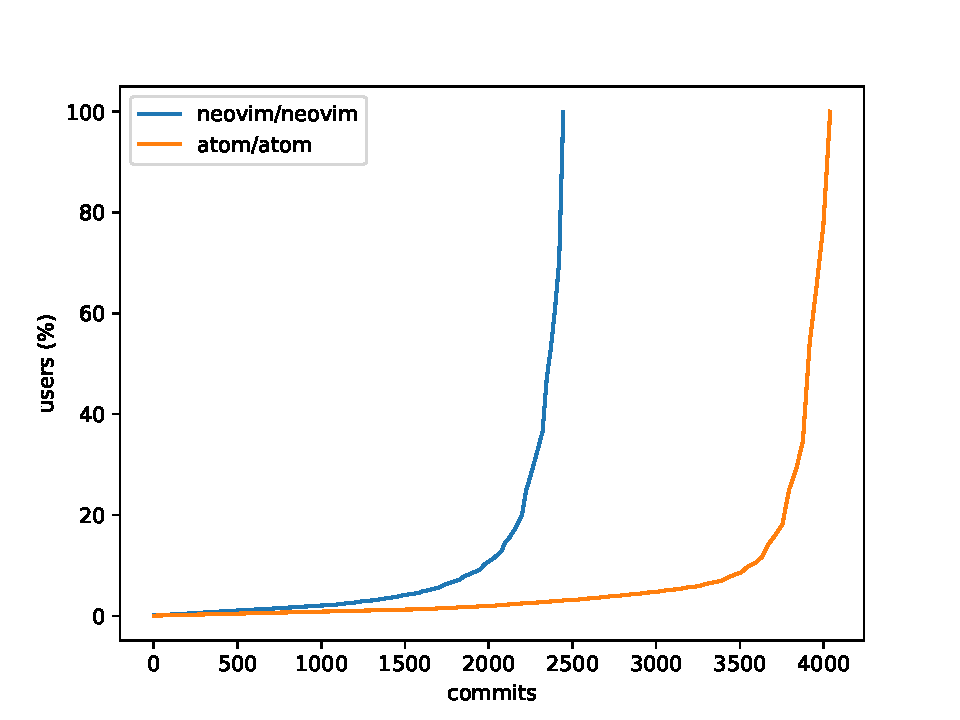
\includegraphics[width=0.7\textwidth]{commits_dist}
	\caption{Commits distribution}
	\label{fig:commits_dist}
\end{figure}
\begin{figure}[!h]
	\centering
	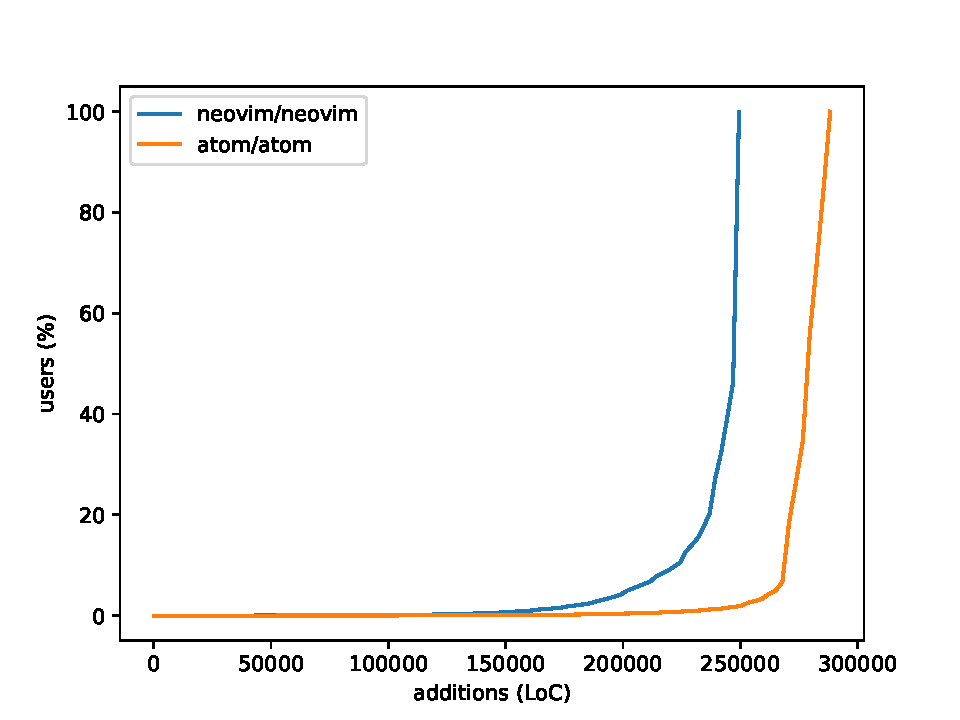
\includegraphics[width=0.7\textwidth]{additions_dist}
	\caption{Additions distribution}	
	\label{fig:additions_dist}
\end{figure}
\begin{figure}[!h]
	\centering
	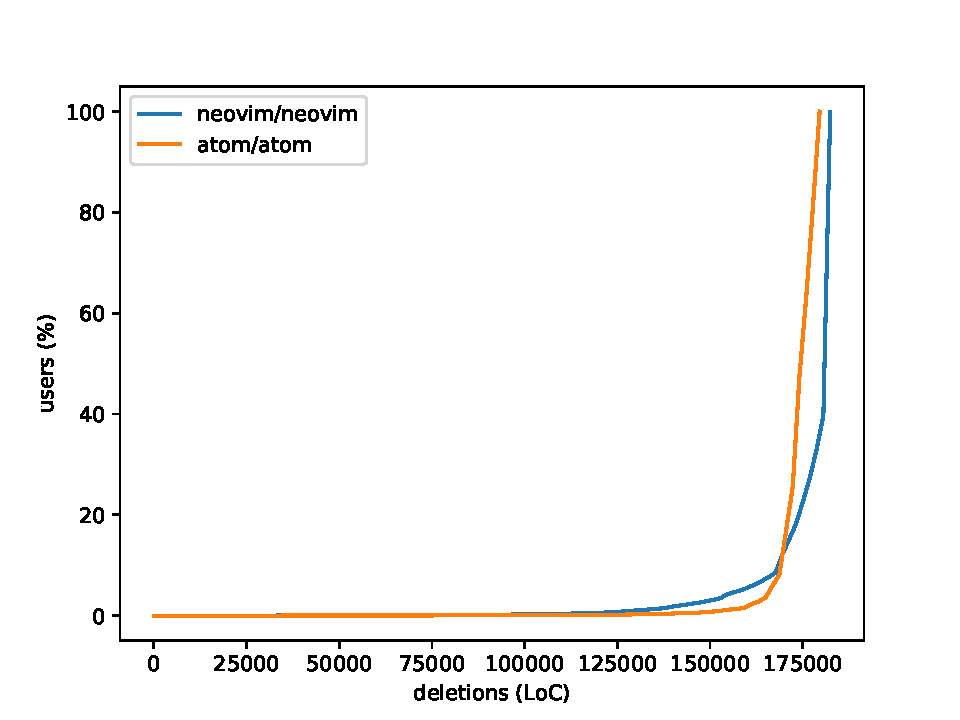
\includegraphics[width=0.7\textwidth]{deletions_dist}
	\caption{Deletions distribution}
	\label{fig:deletions_dist}
\end{figure}

\FloatBarrier
\subsubsection{Feature Proposers \& Problem Reporters}
The amount of feature proposers were ? for the two projects as seen in table~\ref{tab:other_contributors}. The amount of problem reporters were ? for the two projects as seen in table~\ref{tab:other_contributors}. A majority, around 60\%, of the feature proposers and problem reporters did more than one proposal or report and the remaining 40\% did only one report each as seen in figures~\ref{fig:feature_proposers} and ~\ref{fig:problem_reporters}.
\begin{table}[h]
	\centering
	\begin{tabular}{ | l | c | c | }
		\hline
		\textbf{Data Type} 			& \textbf{Atom} 	& \textbf{Neovim}	\\\hline
		Amount of feature proposers	& ?			& ?		 		\\\hline
		Amount of problem reporters	& ?			& ?		 		\\
		\hline 
	\end{tabular}
	\caption{Showing amount of feature proposers.}
	\label{tab:other_contributors}
\end{table}

\begin{figure}[!h]
	\centering
	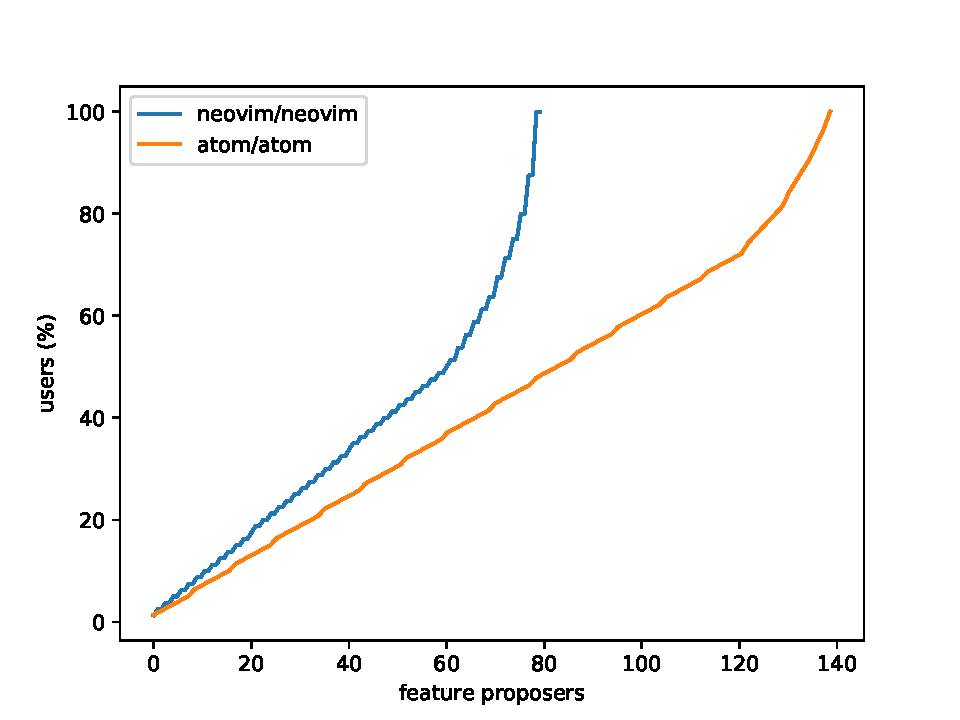
\includegraphics[width=0.7\textwidth]{feature_proposers_dist}
	\caption{Distribution of feature proposals over users.}
	\label{fig:feature_proposers}
\end{figure}
\begin{figure}[!h]
	\centering
	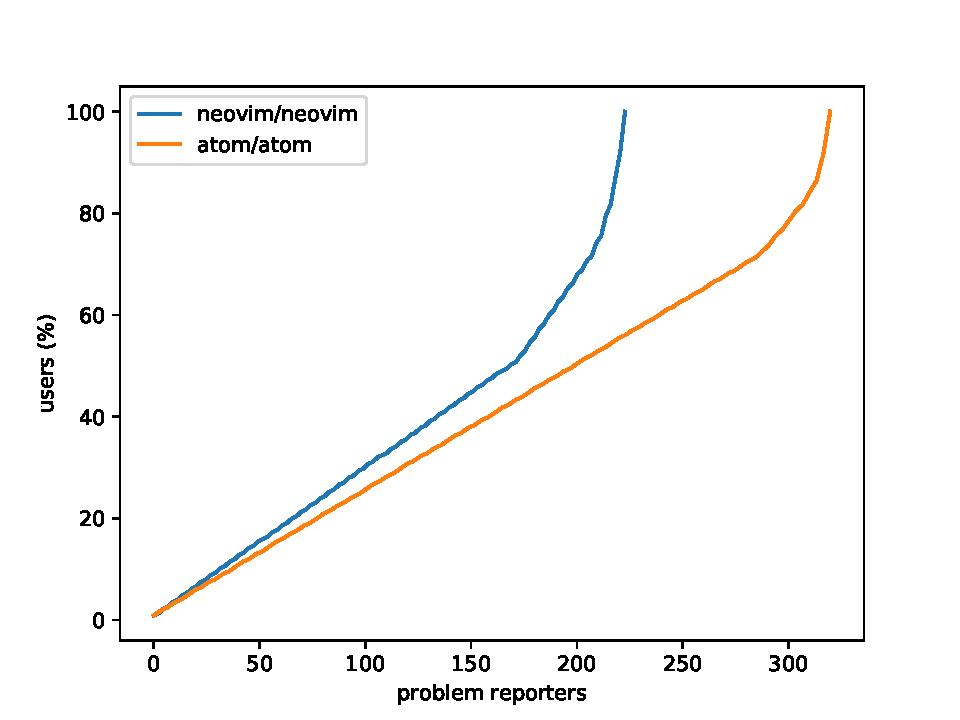
\includegraphics[width=0.7\textwidth]{problem_reporters_dist}
	\caption{Distribution of problem reports over users.}
	\label{fig:problem_reporters}
\end{figure}

\FloatBarrier
\subsubsection{Defect Repair Time}
To two projects differed in the amount of defects repaired and the repair time. With Atom having almost twice as many defects, seen in table ~\ref{tab:defects} and a longer repair time, seen in table~\ref{tab:repair_times}.
\begin{table}[h]
	\centering
	\begin{tabular}{ | l | c | c | }
		\hline
		\textbf{Data Type} 	& \textbf{Atom} 	& \textbf{Neovim}	\\\hline
		Amount defects		& 303		& 153		 	\\
		\hline 
	\end{tabular}
	\caption{Showing amount of reported defects.}
	\label{tab:defects}
\end{table}

\begin{table}[h]
	\centering
	\begin{tabular}{ | l | c | c | }
		\hline
		\textbf{Data Type} 	& \textbf{Atom} 	& \textbf{Neovim}	\\\hline
		Average 			& 185 		& 128 			\\\hline
		Median	 		& 65			& 58 				\\\hline
		Highest			& 1098		& 691			\\\hline
		Lowest			& <1			& <1		 		\\
		\hline 
	\end{tabular}
	\caption{Showing repair time measured in days.}
	\label{tab:repair_times}
\end{table}

\FloatBarrier
\subsection{Sample Data}

\subsubsection{Feature Proposals}
D5
\begin{table}[h]
	\centering
	\begin{tabular}{ | l | c | c | }
		\hline
		\textbf{Username} 	& \textbf{Feature Proposals}	& \textbf{User Status}	\\\hline
		damieng	 		& 3		 				& core dev.			\\\hline
		celrenheit	 		& 2		 				& dev.				\\\hline
		codingbelief	 	& 2		 				& dev.				\\\hline
		fracalo	 		& 2		 				& dev.				\\\hline
		mnquintana	 	& 1		 				& core dev.			\\\hline
		bgriffith	 		& 1		 				& dev.				\\\hline
		caleb531	 		& 1		 				& dev.				\\\hline
		astrojie	 		& 1		 				& dev.				\\\hline
		alhadis	 		& 1		 				& dev.				\\\hline
		kevindeleon	 	& 1		 				& dev.				\\\hline
		MichaelAquiliana	& 1		 				& dev.				\\\hline
		boustanihani	 	& 1		 				& end-user.			\\\hline
		jamesonquinn	 	& 1		 				& end-user.			\\\hline
		jesseleite	 		& 1		 				& end-user			\\\hline
		karai17	 		& 1		 				& end-user			\\
		
		\hline
	\end{tabular}
	\caption{Showing Atom users with amount of feature proposals.}
\end{table}

\begin{table}[h]
	\centering
	\begin{tabular}{ | l | c | c | }
		\hline
		\textbf{Username} 	& \textbf{Feature Proposals}	& \textbf{User Status}	\\\hline
		bfredl			& 4  						& core dev.			\\\hline
		justinmk			& 2  						& core dev.			\\\hline
		tweekmonster 		& 2  						& core dev.			\\\hline
		shougo 			& 2  						& dev.				\\\hline
		Splinterofchaos 	& 1						& core dev.			\\\hline
		jamessan 			& 1  						& core dev.			\\\hline
		elmart 			& 1  						& core dev.			\\\hline
		tarruda 			& 1  						& core dev.			\\\hline
		mtortonesi 		& 1  						& dev.				\\\hline
		shazow 			& 1  						& dev.				\\\hline
		rygwdn 			& 1  						& dev.				\\\hline
		tony 				& 1  						& dev.				\\\hline
		cyphar 			& 1  						& dev.				\\\hline
		joshtriplett 		& 1  						& dev.				\\\hline
		nhooyr 			& 1  						& dev.				\\\hline
		ZyX-I 			& 1  						& dev.				\\\hline
		equalsraf			& 1		 				& dev.				\\\hline
		sunaku 			& 1  						& end-user.			\\\hline
		abstiles			& 1		 				& end-user.			\\\hline
		mmlb 			& 1  						& end-user.			\\
		\hline
	\end{tabular}
	\caption{Showing Neovim users with amount of feature proposals.}
\end{table}
\begin{table}[h]
	\centering
	\begin{tabular}{ | l | c | c | }
		\hline
		\textbf{User Group} 	& \textbf{Atom} 	& \textbf{Neovim}	\\\hline
		core devs 			& 2 			& 7 				\\\hline
		devs	 			& 9			& 10 				\\\hline
		end-users			& 4			& 3				\\
		\hline
	\end{tabular}
	\caption{Showing amount of feature proposers in user groups.}
\end{table}

\FloatBarrier
\subsubsection{Feature Origin Categories}
D6
\begin{table}[h]
	\centering
	\begin{tabular}{ | l | c | c | c | c |}
		\hline
		\textbf{Proposal Category} 	& \textbf{Atom} 	& \textbf{Neovim}	\\\hline
		A						& 16 			& 18				\\\hline
		B		 				& 2			& 6 	 			\\\hline
		C						& 4			& 3				\\\hline
		tot. 						& 22 			& 27 				\\
		\hline
	\end{tabular}
	\caption{Showing amount of proposals for each category.}
\end{table}

\FloatBarrier
\subsubsection{Feature Acknowledgement}
D7
\begin{table}[h]
	\centering
	\begin{tabular}{ | l | c | c | }
		\hline
		\textbf{Username} 	& \textbf{Feature Acknowledgements}	& \textbf{User Status}	\\\hline
		fracalo 			& 4  								& dev.				\\\hline
		bastillian 			& 3  								& dev.				\\\hline
		kuychaco 			& 2  								& core dev.			\\\hline
		damieng 			& 2  								& core dev.			\\\hline
		50Wliu 			& 2  								& core dev.			\\\hline
		svanharmelen 		& 2  								& dev.				\\\hline
		as-cii 			& 1  								& core dev.			\\\hline
		lee-dohm 			& 1  								& core dev.			\\\hline
		simurai 			& 1  								& core dev.			\\\hline
		izuzak 			& 1  								& core dev.			\\\hline
		codingbelief 		& 1 								& dev.			  	\\\hline
		benogle 			& 1  								& dev.				\\\hline
		nathansobo 		& 1  								& dev.				\\
		\hline
	\end{tabular}
	\caption{Showing Atom users with amount of feature acknowledgements.}
\end{table}
\begin{table}[h]
	\centering
	\begin{tabular}{ | l | c | c | }
		\hline
		\textbf{Username} 	& \textbf{Feature Acknowledgements}	& \textbf{User Status}	\\\hline
		justinmk 			& 12  							& core dev.			\\\hline
		bfredl 			& 4	 							& core dev.			\\\hline
		tarruda 			& 2  								& core dev.			\\\hline
		jamessan 			& 2  								& core dev.			\\\hline
		tweekmonster 		& 2  								& core dev.			\\\hline
		alexgenco 		& 2  								& dev.				\\\hline
		mhinz 			& 1  								& core dev.			\\\hline
		tjdevries			& 1  								& dev.				\\\hline
		shougo 			& 1  								& dev.				\\
		\hline
	\end{tabular}
	\caption{Showing Neovim users with amount of feature acknowledgements.}
\end{table}

\FloatBarrier
\subsubsection{First Implementation of Feature}
D8
\begin{table}[h]
	\centering
	\begin{tabular}{ | l | c | c | }
		\hline
		\textbf{Username} 	& \textbf{First Feature Implementations}	& \textbf{User Status}	\\\hline
		damieng 			& 3  								& core dev.			\\\hline
		bastillian 			& 3  								& dev.				\\\hline		
		50Wliu			& 1  								& core dev.			\\\hline
		kuychaco 			& 1  								& core dev.			\\\hline
		wil93 			& 1  								& core dev.			\\\hline
		alhadis 			& 1  								& dev.				\\\hline
		astrojie 			& 1  								& dev.				\\\hline
		caleb531 			& 1  								& dev.			 	\\\hline
		codingbelief 		& 1 								& dev.			  	\\\hline
		danjordan 		& 1  								& dev.			 	\\\hline
		esdoppio 			& 1  								& dev.				\\\hline
		fracalo 			& 1  								& dev.				\\\hline
		jtokoph 			& 1  								& dev.				\\\hline
		kevindeleon 		& 1  								& dev.				\\\hline
		MichaelAquilina 	& 1  								& dev.				\\\hline
		timkelty 			& 1  								& dev.				\\
		\hline
	\end{tabular}
	\caption{Showing Atom users with amount of first feature implementations.}
\end{table}
\begin{table}[h]
	\centering
	\begin{tabular}{ | l | c | c | }
		\hline
		\textbf{Username} 	& \textbf{First Feature Implementations}	& \textbf{User Status}	\\\hline
		justinmk			& 10  							& core dev.			\\\hline
		bfredl			& 8  								& core dev.			\\\hline
		tweekmonster		& 2  								& core dev.			\\\hline
		jamessan			& 2  								& core dev.			\\\hline
		alexgenco			& 1		 						& dev				\\\hline
		nhooyr			& 1  								& dev.				\\\hline
		shougo			& 1  								& dev.				\\\hline
		ZyX-I			& 1		 						& dev.				\\
		\hline
	\end{tabular}
	\caption{Showing Neovim users with amount of first feature implementations.}
\end{table}

\FloatBarrier
\section{Analysis}

\section{Discussion}

\section{Conclusion and Suggestions for Future Work} % TODO Conlusion and Related Work as separate sections?

\newpage
\addcontentsline{toc}{section}{References}
\bibliographystyle{plain}
\bibliography{library,custom}

\end{document}
